\begin{example}[פאזל הזזה]
נתון לוח משחק בגודל 
$n \times m$
על הלוח 
$nm - 1$
חלקים ממוספרים מ-1 עד 
$nm - 1$
ומשבצת ריקה.
נתון סידור ראשוני של החלקים ואנו רוצים לסדר את החלקים לפי הסדר 
כך שבכל שלב מותר לנו להזיז את אחד החלקים ששכנים למשבצת הריקה אל המשבצת הריקה.
\end{example}
למשל עבור
$n = m = 3$:
\begin{center}
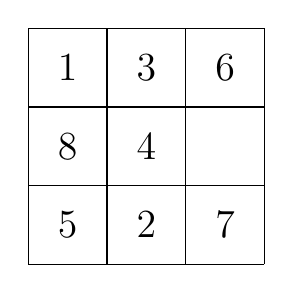
\begin{tikzpicture}
\draw (0,0) grid (3,3);

\begin{scope}[xshift=.5cm, yshift=.5cm, font=\Large]
\foreach \x \y \i in {0/0/5, 1/0/2, 2/0/7, 0/1/8, 1/1/4, 0/2/1, 1/2/3, 2/2/6}{
	\node at(\x, \y) {\i};
}
\end{scope}

\end{tikzpicture}
\end{center}


הציעו אלגוריתם לפתרון הבעיה.
